\documentclass [norsk,a4paper,twoside]{article}\usepackage[]{graphicx}\usepackage[]{color}
%% maxwidth is the original width if it is less than linewidth
%% otherwise use linewidth (to make sure the graphics do not exceed the margin)
\makeatletter
\def\maxwidth{ %
  \ifdim\Gin@nat@width>\linewidth
    \linewidth
  \else
    \Gin@nat@width
  \fi
}
\makeatother

\definecolor{fgcolor}{rgb}{0.345, 0.345, 0.345}
\newcommand{\hlnum}[1]{\textcolor[rgb]{0.686,0.059,0.569}{#1}}%
\newcommand{\hlstr}[1]{\textcolor[rgb]{0.192,0.494,0.8}{#1}}%
\newcommand{\hlcom}[1]{\textcolor[rgb]{0.678,0.584,0.686}{\textit{#1}}}%
\newcommand{\hlopt}[1]{\textcolor[rgb]{0,0,0}{#1}}%
\newcommand{\hlstd}[1]{\textcolor[rgb]{0.345,0.345,0.345}{#1}}%
\newcommand{\hlkwa}[1]{\textcolor[rgb]{0.161,0.373,0.58}{\textbf{#1}}}%
\newcommand{\hlkwb}[1]{\textcolor[rgb]{0.69,0.353,0.396}{#1}}%
\newcommand{\hlkwc}[1]{\textcolor[rgb]{0.333,0.667,0.333}{#1}}%
\newcommand{\hlkwd}[1]{\textcolor[rgb]{0.737,0.353,0.396}{\textbf{#1}}}%
\let\hlipl\hlkwb

\usepackage{framed}
\makeatletter
\newenvironment{kframe}{%
 \def\at@end@of@kframe{}%
 \ifinner\ifhmode%
  \def\at@end@of@kframe{\end{minipage}}%
  \begin{minipage}{\columnwidth}%
 \fi\fi%
 \def\FrameCommand##1{\hskip\@totalleftmargin \hskip-\fboxsep
 \colorbox{shadecolor}{##1}\hskip-\fboxsep
     % There is no \\@totalrightmargin, so:
     \hskip-\linewidth \hskip-\@totalleftmargin \hskip\columnwidth}%
 \MakeFramed {\advance\hsize-\width
   \@totalleftmargin\z@ \linewidth\hsize
   \@setminipage}}%
 {\par\unskip\endMakeFramed%
 \at@end@of@kframe}
\makeatother

\definecolor{shadecolor}{rgb}{.97, .97, .97}
\definecolor{messagecolor}{rgb}{0, 0, 0}
\definecolor{warningcolor}{rgb}{1, 0, 1}
\definecolor{errorcolor}{rgb}{1, 0, 0}
\newenvironment{knitrout}{}{} % an empty environment to be redefined in TeX

\usepackage{alltt}
\addtolength{\hoffset}{-0.5cm}
\addtolength{\textwidth}{1cm}
\addtolength{\voffset}{-1cm}
\addtolength{\textheight}{2cm}


%for nice looking tabs
\usepackage{booktabs}

\usepackage[norsk]{babel}
\usepackage[utf8x]{inputenc}
\usepackage{textcomp}
\usepackage{fancyhdr}
\pagestyle{fancy}
\usepackage{amsmath}
\usepackage{rotating} %add rotating for plain tables
\usepackage{pdflscape} %add rotating/landcape for pdf

%add rotating for plain tables
\usepackage{rotating}

%add rotating/landcape for pdf
\usepackage{pdflscape}

%bytte font
\renewcommand{\familydefault}{\sfdefault}

%setter grå skrift fremfort sort
\usepackage{xcolor}
\usepackage{graphicx}
\usepackage[pdftex, colorlinks, linkcolor=OffBlaa3, urlcolor=OffBlaa3]{hyperref}
\IfFileExists{upquote.sty}{\usepackage{upquote}}{}
\begin{document}








\section{Oppsummeringstall for NKR}

% latex table generated in R 3.4.1 by xtable 1.8-2 package
% Sun Aug 20 20:04:28 2017
\begin{table}[ht]
\centering
\begin{tabular}{lrrrrrr}
  \hline
 & 2012 & 2013 & 2014 & 2015 & 2016 & Sum \\ 
  \hline
Ahus & 50 & 151 & 67 & 136 & 184 & 605 \\ 
  Aleris, Bergen & 217 & 265 & 145 & 95 & 59 & 939 \\ 
  Aleris, Oslo & 152 & 4 & 38 & 190 & 72 & 773 \\ 
  Arendal & 84 & 95 & 87 & 82 & 72 & 558 \\ 
  Bodø & 5 & 0 & 0 & 27 & 20 & 88 \\ 
  Bærum & 79 & 88 & 65 & 111 & 134 & 612 \\ 
  Drammen & 148 & 102 & 186 & 249 & 273 & 1108 \\ 
  Elverum & 94 & 127 & 147 & 139 & 128 & 887 \\ 
  Flekkefjord & 12 & 10 & 2 & 8 & 6 & 53 \\ 
  Førde & 0 & 0 & 0 & 0 & 25 & 32 \\ 
  Gjøvik & 85 & 74 & 94 & 75 & 118 & 643 \\ 
  Haugesund & 5 & 38 & 54 & 42 & 82 & 221 \\ 
  Haukeland, nevrokir & 158 & 170 & 186 & 168 & 170 & 1001 \\ 
  Haukeland, ort & 4 & 0 & 1 & 18 & 23 & 50 \\ 
  Ibsensykehuset & 0 & 0 & 0 & 0 & 1 & 1 \\ 
  Kolibri Medical Group & 0 & 18 & 3 & 0 & 0 & 21 \\ 
  Kristiansand & 96 & 112 & 110 & 137 & 165 & 788 \\ 
  Kristiansund & 0 & 0 & 0 & 0 & 34 & 34 \\ 
  Kysthospitalet Hagevik & 202 & 244 & 269 & 275 & 291 & 1698 \\ 
  Larvik & 29 & 0 & 0 & 0 & 117 & 202 \\ 
  Levanger & 75 & 99 & 112 & 116 & 109 & 659 \\ 
  Lillehammer & 91 & 61 & 62 & 99 & 77 & 511 \\ 
  Martina Hansens & 319 & 270 & 304 & 341 & 307 & 2006 \\ 
  Namsos & 64 & 55 & 93 & 73 & 71 & 430 \\ 
  NIMI & 27 & 24 & 129 & 111 & 116 & 458 \\ 
  Oslofjordklinikken Vest & 0 & 0 & 6 & 59 & 96 & 161 \\ 
  Oslofjordklinikken Øst & 266 & 303 & 345 & 341 & 324 & 1943 \\ 
  Rana & 10 & 19 & 23 & 23 & 30 & 145 \\ 
  Rikshospitalet, nevrokir & 37 & 52 & 55 & 63 & 33 & 400 \\ 
  Rikshospitalet, ort & 15 & 4 & 2 & 0 & 0 & 22 \\ 
  Skien & 1 & 23 & 41 & 39 & 66 & 170 \\ 
  St.Olavs, nevrokir & 345 & 325 & 346 & 356 & 299 & 2259 \\ 
  St.Olavs, ort & 58 & 46 & 50 & 32 & 39 & 350 \\ 
  Stavanger, nevrokir & 212 & 200 & 172 & 156 & 131 & 979 \\ 
  Stavanger, ort & 231 & 234 & 237 & 274 & 270 & 1331 \\ 
  Teres Colloseum, Oslo & 5 & 41 & 26 & 26 & 79 & 192 \\ 
  Teres Colloseum, Stavanger & 0 & 0 & 31 & 46 & 32 & 159 \\ 
  Teres, Bergen & 0 & 0 & 0 & 0 & 0 & 15 \\ 
  Teres, Drammen & 43 & 37 & 0 & 0 & 0 & 138 \\ 
  Ullevål, nevrokir & 34 & 80 & 30 & 42 & 88 & 274 \\ 
  Ullevål, ort & 117 & 136 & 126 & 162 & 166 & 955 \\ 
  Ulriksdal & 92 & 9 & 0 & 0 & 0 & 338 \\ 
  UNN, nevrokir & 275 & 221 & 222 & 245 & 206 & 1759 \\ 
  Volda & 24 & 29 & 27 & 38 & 31 & 170 \\ 
  Volvat & 0 & 21 & 80 & 139 & 136 & 377 \\ 
  Østfold & 0 & 0 & 61 & 48 & 44 & 153 \\ 
  Ålesund & 105 & 103 & 127 & 102 & 109 & 747 \\ 
  Sum & 3866 & 3890 & 4161 & 4683 & 4833 & 27415 \\ 
   \hline
\end{tabular}
\caption{Antall registreringer ved hver avdeling siste 5 år, samt totalt siden 2010.} 
\label{tab:AntReg}
\end{table}


Tabell \ref{tab:AntReg} viser antall 
registreringer gjort ved de respektive avdelinger hvert år. Vi ser at det er  
47 avdelinger som registrerer og at det i perioden 2010 til 2016 totalt er registrert 27415 
operasjoner. Av disse er 53.1\% utført på menn og 46.9\% på kvinner.
Siste inngrep registrert i datauttrekket som ligger til grunn for denne rapporten, ble utført 
2016-12-30. 
\par 
\clearpage



\section{Bakgrunnsdata}
\subsection{Aldersfordeling}


% latex table generated in R 3.4.1 by xtable 1.8-2 package
% Sun Aug 20 20:04:28 2017
\begin{table}[ht]
\centering
\begin{tabular}{rlllllllll}
  \hline
 & 0-19 & 20-29 & 30-39 & 40-49 & 50-59 & 60-69 & 70-79 & 80-89 & 90+ \\ 
  \hline
Andeler & 0.4\% & 4.5\% & 11.8\% & 18.7\% & 20.3\% & 21\% & 18.9\% & 4.3\% & 0.1\% \\ 
  Antall & 21 & 216 & 569 & 898 & 976 & 1013 & 909 & 207 & 4 \\ 
   \hline
\end{tabular}
\caption{Aldersfordeling.} 
\label{tab:Alder}
\end{table}


Figur \ref{fig:Alder} viser aldersfordeling for alle pasienter i 2016.
De nøyaktige tallene for aldersfordelinga framgår av Tabell \ref{tab:Alder}. 


\begin{figure}[ht]
	\centering 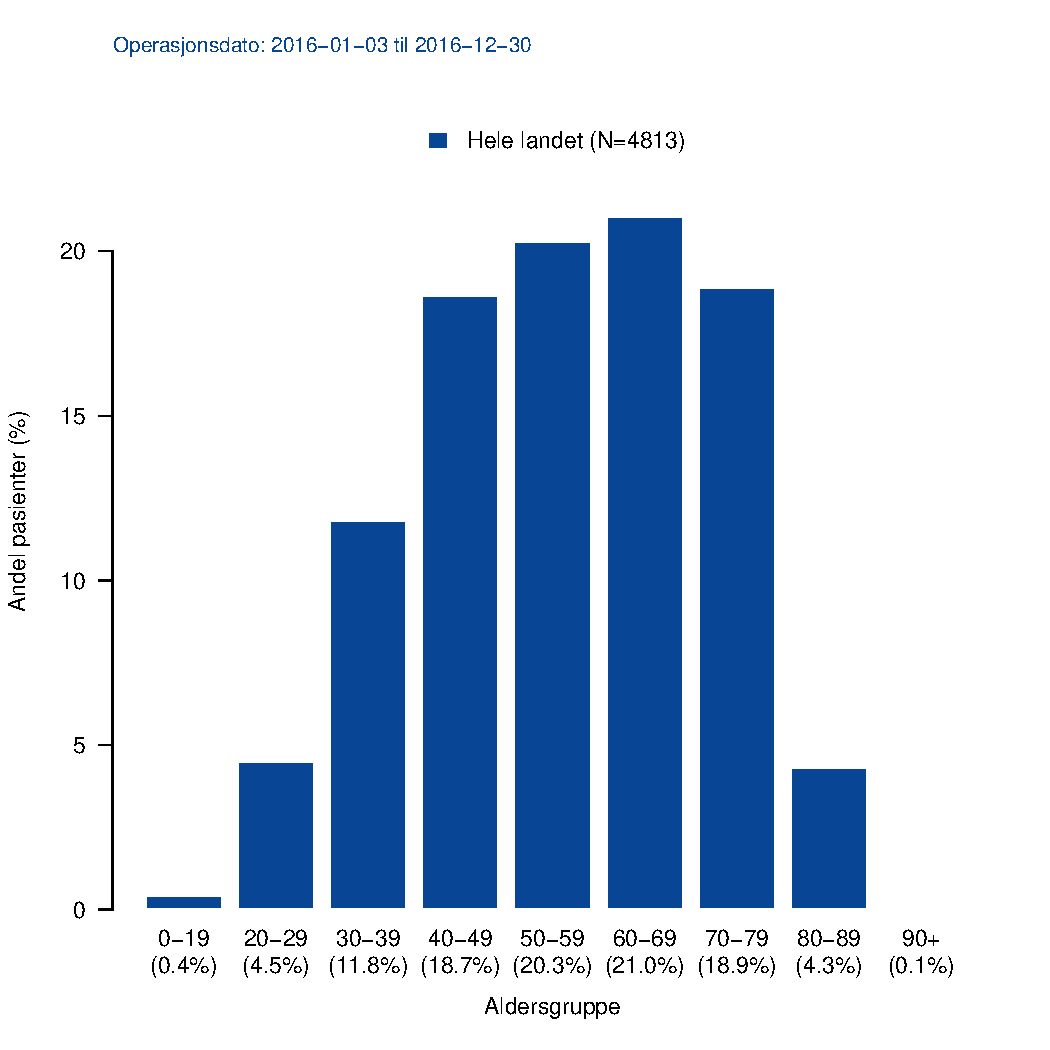
\includegraphics[width= 0.8\textwidth]{FigAlderFord.pdf}
	\caption{\label{fig:Alder} Aldersfordeling., 2016}
\end{figure}


\subsection{Sivilstatus}
Tabell \ref{tab:SivStat} viser sivilstatus for alle som ble opererte i 2016

% latex table generated in R 3.4.1 by xtable 1.8-2 package
% Sun Aug 20 20:04:28 2017
\begin{table}[ht]
\centering
\begin{tabular}{lrr}
  \hline
 & Antall & Andeler \\ 
  \hline
Gift & 2734 & 56.8\% \\ 
  Samboer & 805 & 16.7\% \\ 
  Enslig & 1250 & 26\% \\ 
  Ikke svart & 24 & 0.5\% \\ 
  Tot. ant. & 4813 &  \\ 
   \hline
\end{tabular}
\caption{Sivilstatus for opererte pasienter} 
\label{tab:SivStat}
\end{table}



\subsection{Morsmål / etnisitet}

% latex table generated in R 3.4.1 by xtable 1.8-2 package
% Sun Aug 20 20:04:28 2017
\begin{table}[ht]
\centering
\begin{tabular}{lrr}
  \hline
 & Antall & Andeler \\ 
  \hline
Norsk & 4509 & 93.7\% \\ 
  Samisk & 5 & 0.1\% \\ 
  Annet & 277 & 5.8\% \\ 
  Ikke svart & 22 & 0.5\% \\ 
   \hline
\end{tabular}
\caption{Pasientenes morsmål} 
\label{tab:Morsm}
\end{table}


Tabell \ref{tab:Morsm} viser fordeling av norske, samiske og andre fremmedsåpråklige pasienter.
% for alle som ble operert ved shtxt sammenliknet med landet for øvrig. 
Andel fremmedspråklige 
pasienter (inkl. samisk) var 5.9\% . 


\subsection{Utdanning}
Figur \ref{fig:Utd} viser nivå av utdanning 
Opplysningene om utdanning er rapportert av pasientene selv.



\begin{figure}[ht]
	\centering 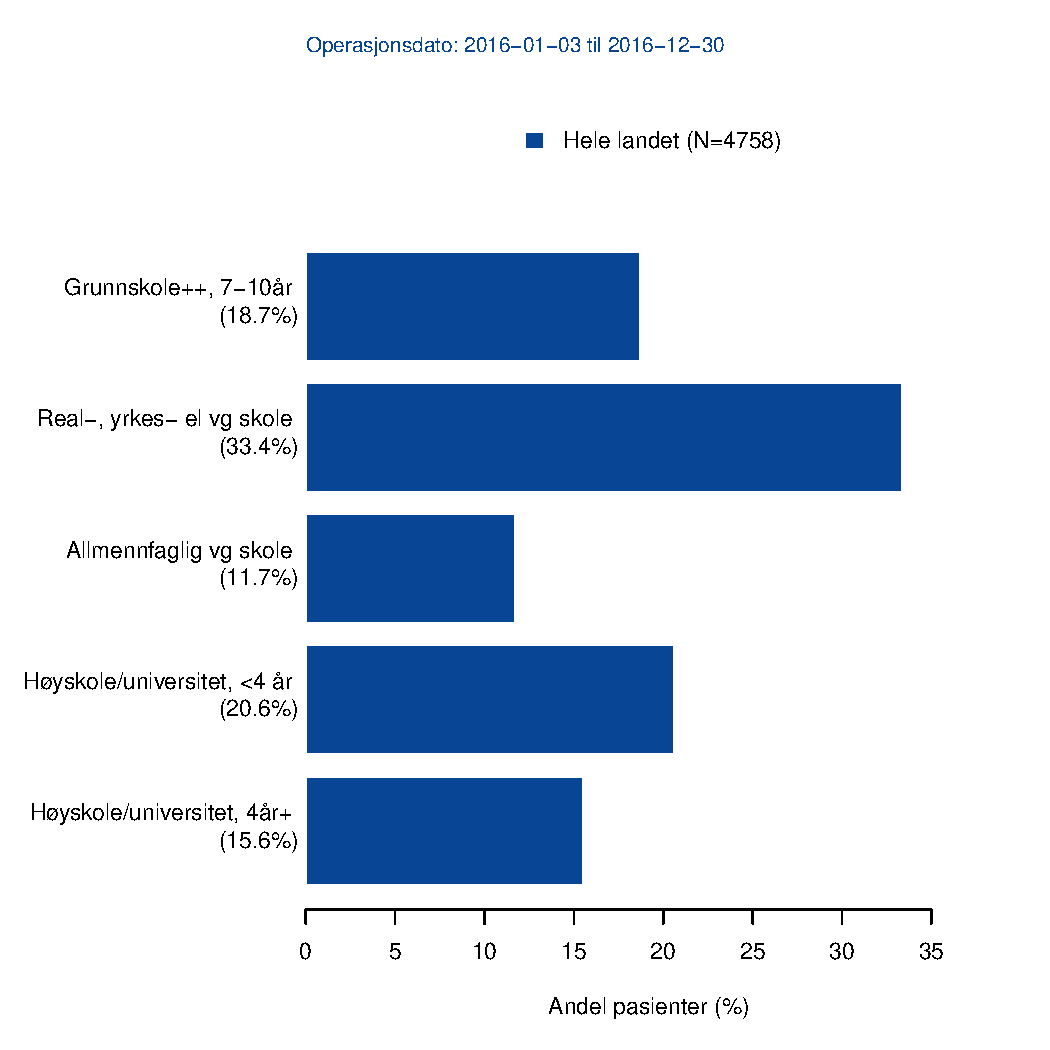
\includegraphics[width= 0.8\textwidth]{FigUtd.pdf}
	\caption{\label{fig:Utd} Høyeste fullførte utdanning.}
\end{figure}


\subsection{Røyking}


Det er 21\% av mennene og 22\% av kvinnene som røyker. 
Total andel røykere er 21\%


\subsection{Arbeidsstatus}

% latex table generated in R 3.4.1 by xtable 1.8-2 package
% Sun Aug 20 20:04:29 2017
\begin{table}[ht]
\centering
\begin{tabular}{lr}
  \hline
 & Andeler \\ 
  \hline
I arbeid & 19.2\% \\ 
  Hjemmeværende & 1.6\% \\ 
  Student/skoleelev & 1.2\% \\ 
  Pensjonist & 28.8\% \\ 
  Arbeidsledig & 1.4\% \\ 
  Sykemeldt & 22.9\% \\ 
  Aktiv sykemeldt & 1.1\% \\ 
  Delvis Sykemeldt & 7.9\% \\ 
  Attføring/rehabiliteirng & 4.2\% \\ 
  Uføretrygdet & 11.6\% \\ 
   \hline
\end{tabular}
\caption{Arbeidsstatus} 
\label{tab:Arb}
\end{table}


Tabell \ref{tab:Arb} viser fordeling av arbeidsstatus før operasjon for de 98.1\% 
av pasientene som har svart på spørsmål om arbeidsstatus.
Andelen pasienter som mottok sykepenger (sykemeldte, uføretrygdede eller personer 
på attføring) og av den grunn var helt eller delvis ute av jobb før operasjonen (preop) var 
47.7 \%. 
Median varighet av sykemelding/attføring/rehabilitering  før operasjon var 
15 uker.


\clearpage


\subsection{Uføretrygd og erstatning }

Tabell \ref{tab:Ufor} viser pasientenes svar på spørsmålet: ``Har du søkt om uføretrygd?''.

% latex table generated in R 3.4.1 by xtable 1.8-2 package
% Sun Aug 20 20:04:29 2017
\begin{table}[ht]
\centering
\begin{tabular}{lr}
  \hline
 & Andeler \\ 
  \hline
Ja & 2\% \\ 
  Nei & 75.2\% \\ 
  Planlegger å søke & 2.2\% \\ 
  Er innvilget & 11.5\% \\ 
  Ikke besvart & 9.1\% \\ 
   \hline
\end{tabular}
\caption{Spørsmål: Har du søkt om uføretrygd?} 
\label{tab:Ufor}
\end{table}



Tabell \ref{tab:Erst} viser pasientenes svar på spørsmålet: ``Har du søkt om erstatning?'' 

% latex table generated in R 3.4.1 by xtable 1.8-2 package
% Sun Aug 20 20:04:29 2017
\begin{table}[ht]
\centering
\begin{tabular}{lr}
  \hline
 & Andeler \\ 
  \hline
Ja & 2.6\% \\ 
  Nei & 87.6\% \\ 
  Planlegger å søke & 1.8\% \\ 
  Er innvilget & 2.1\% \\ 
  Ikke besvart & 5.9\% \\ 
   \hline
\end{tabular}
\caption{Spørsmål: Har du søkt om erstatning fra forsikringsselskap eller folketrygden, 
		eventuelt yrkesskadeerstatning)?} 
\label{tab:Erst}
\end{table}



\subsection{Tidligere ryggoperert}
Informasjonen er hentet fra legeskjema.
Figur \ref{fig:TidlOp} viser en prosentvis fordelig mellom primæroperasjon, det vil si første gangs 
operasjon, og operasjoner hos pasienter som har vært operert tidligere.  
Søylene representerer hvert år frem til i dag. Tallet på toppen av søylen viser antall operasjoner utført 
det aktuelle året.



\begin{figure}[ht]
	\centering 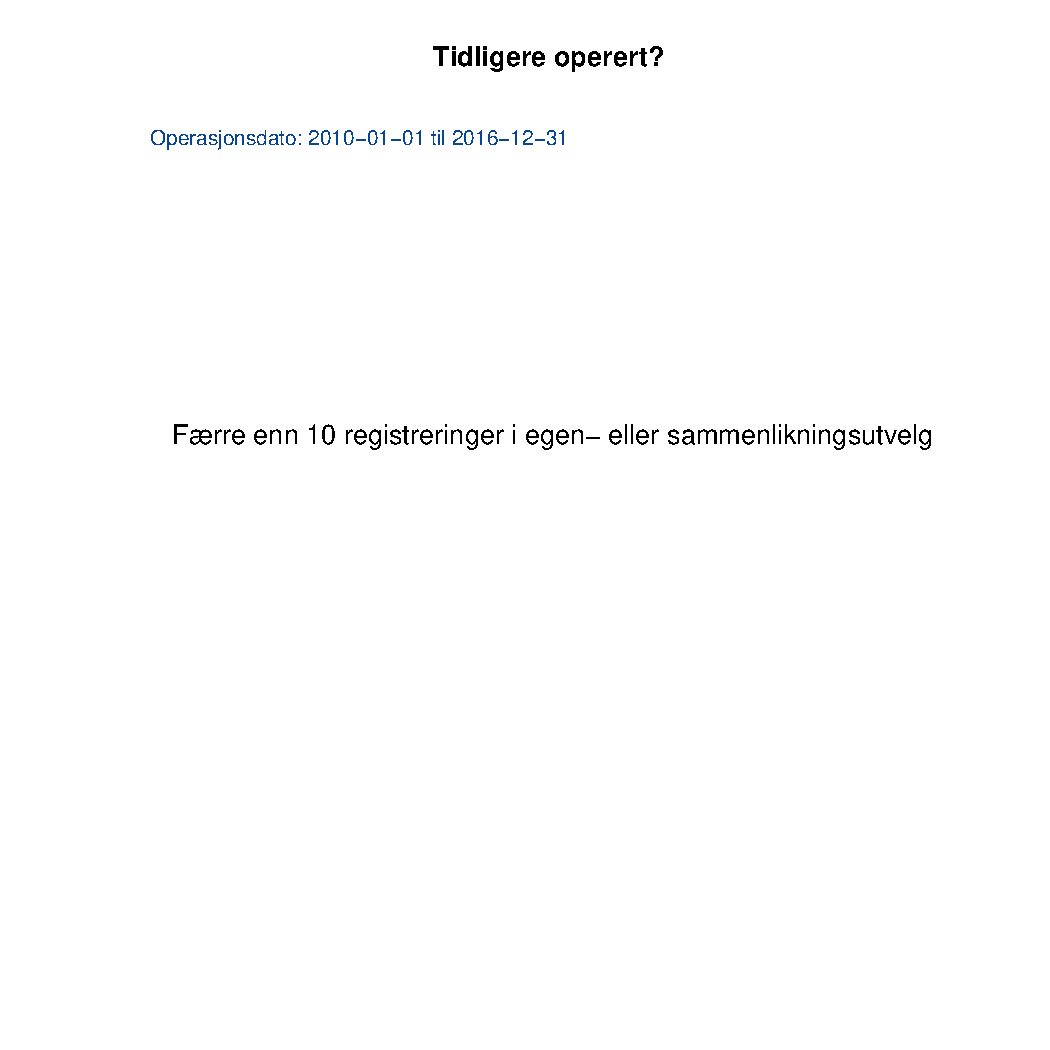
\includegraphics[width= 0.8\textwidth]{TidlOp.pdf}
	\caption{\label{fig:TidlOp} Tidligere operert? }
\end{figure}



Av de pasientene som hadde vært operert tidligere var 63.2\% 
operert i samme nivå, 31.3\% 
operert i annet nivå og 5.5\% 
operert i både samme og annet nivå. 
(\textit{Dette gjelder hele tidsperioden. Skal disse resultatene være med, må de gjelde kun 2016.})


\subsection{Kroppsmasseindex (Body Mass Index, BMI)}
Opplysninger om høyde og vekt er rapportert fra pasientene selv. BMI er gitt ved:
\begin{equation*}
	\text{BMI} = \frac{\text{Vekt}(kg)}{\text{Høyde}^2 (m^2)}
\end{equation*} 

Figur \ref{fig:BMI} viser fordeling av BMI for alle pasienter i 2016. 
%operert ved shtxt sammenlignet med pasienter fra resten av landet.




\begin{figure}[ht]
	\centering 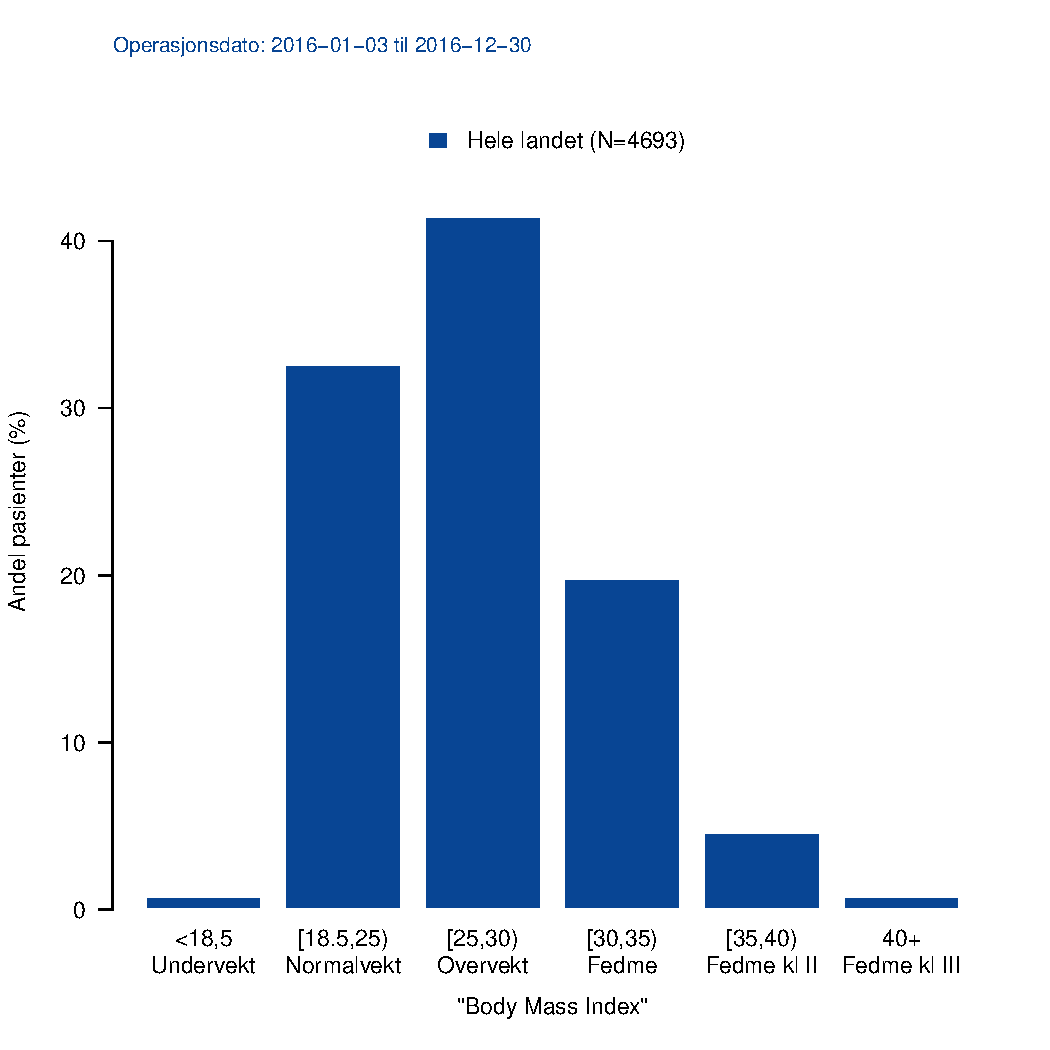
\includegraphics[width= 0.8\textwidth]{FigBMI.pdf}
	\caption{\label{fig:BMI} Pasientenes BMI (Body Mass Index).}
\end{figure}



\clearpage


\subsection{Varighet av smerter i rygg-/hofte og av utstrålende smerter på operasjonstidspunktet}

% latex table generated in R 3.4.1 by xtable 1.8-2 package
% Sun Aug 20 20:04:30 2017
\begin{table}[ht]
\centering
\begin{tabular}{lr}
  \hline
 & Andeler \\ 
  \hline
Ingen rygg-/hoftesmerter & 1.7\% \\ 
  $<$ 3 mnd & 9\% \\ 
  3 - 12 mnd & 30.8\% \\ 
  1 - 2 år & 16.5\% \\ 
  $>$ 2 år & 38.2\% \\ 
  Ikke besvart & 3.8\% \\ 
   \hline
\end{tabular}
\caption{Varighet av rygg-/hoftesmerter på operasjonstidspunktet} 
\label{tab:SmRH}
\end{table}
% latex table generated in R 3.4.1 by xtable 1.8-2 package
% Sun Aug 20 20:04:30 2017
\begin{table}[ht]
\centering
\begin{tabular}{lr}
  \hline
 & Andeler \\ 
  \hline
Ingen utstrålende smerter & 2.7\% \\ 
  $<$ 3 mnd & 13.5\% \\ 
  3 - 12 mnd & 35\% \\ 
  1 - 2 år & 17.5\% \\ 
  $>$ 2 år & 26.2\% \\ 
  Ikke besvart & 5.2\% \\ 
   \hline
\end{tabular}
\caption{Varighet av nåværende utstrålende smerter} 
\label{tab:Utstr}
\end{table}

Spørsmålene er besvart av pasienten.
Tabellene \ref{tab:SmRH}  og \ref{tab:Utstr} viser fordeling av hvor lenge pasientene har hatt 
hhv. smerter i rygg/hofte og utstrålende smerter.

\textit{NB: Fix så det blir 1 desimal i alle tall}



\begin{figure}[h] 
  \scalebox{0.8}{\includegraphics{VarighUtstrAvd.pdf}}
  \caption{Prolapspasienter som har utstrålende smerter
			i mer enn ett år før operasjonen.}
  \label{fig:VarighSmerteUtstrAvd}
\end{figure}

\begin{figure}[h] 
  \scalebox{0.8}{\includegraphics{VarighRyggHofAvd.pdf}}
  \caption{Prolapspasienter som har hatt smerter i rygg-/hofte
			i mer enn ett år før operasjonen.}
  \label{fig:VarighSmerteRyggAvd}
\end{figure}


\subsection{ASA-grad}
%Tabell, figur eller begge deler?
ASA angir pasientens ”sårbarhet” i forhold til å få anestesi og operasjon på en skala fra 1 til 5. 
Opplysningene skal hentes fra anestesiskjema som fylles ut av anestesilege/sykepleier før operasjon.
%For hele landet:
Tabell \ref{tab:ASA} viser fordeling av ASA grad. Andelen pasienter med ASA grad I-II 
var 85.6\%. 


% latex table generated in R 3.4.1 by xtable 1.8-2 package
% Sun Aug 20 20:04:31 2017
\begin{table}[ht]
\centering
\begin{tabular}{crr}
  \hline
 & Antall & Prosent \\ 
  \hline
I & 1334 & 27.7\% \\ 
  II & 2787 & 57.9\% \\ 
  III & 657 & 13.7\% \\ 
  IV & 5 & 0.1\% \\ 
  Ikke besvart & 30 & 0.6\% \\ 
   \hline
\end{tabular}
\caption{Fordeling av ASA-grad} 
\label{tab:ASA}
\end{table}




\subsection{Radiologisk utredning}
\subsubsection{Radiologisk vurdering}

% latex table generated in R 3.4.1 by xtable 1.8-2 package
% Sun Aug 20 20:04:31 2017
\begin{table}[ht]
\centering
\begin{tabular}{lrr}
  \hline
 & Antall & Andeler \\ 
  \hline
CT & 339 & 7\% \\ 
  MR & 4712 & 97.9\% \\ 
  Radikulografi & 33 & 0.7\% \\ 
  Diskografi & 2 & 0\% \\ 
  Diagnostisk blokade & 12 & 0.2\% \\ 
  Røntgen LS-columna & 1043 & 21.7\% \\ 
  Med fleksjon/ekstensjon & 335 & 7\% \\ 
  Tot. ant. & 4813 &   \\ 
   \hline
\end{tabular}
\caption{Radiologisk vurdering, 2016} 
\label{tab:RV}
\end{table}


Tabell \ref{tab:RV} viser hvor stor andel av pasientene som har vært til ulike typer 
radiologisk undersøkelse. 
Spørsmålene er besvart av leger. En pasient kan ha vært til flere undersøkelser.


\subsubsection{Radiologiske funn/diagnoser}


% latex table generated in R 3.4.1 by xtable 1.8-2 package
% Sun Aug 20 20:04:31 2017
\begin{table}[ht]
\centering
\begin{tabular}{lrr}
  \hline
 & Antall & Andeler \\ 
  \hline
Skiveprolaps & 2206 & 45.8\% \\ 
  Sentral spinalstenose & 1498 & 31.1\% \\ 
  Lateral spinalstenose & 1578 & 32.8\% \\ 
  Foraminal stenose & 590 & 12.3\% \\ 
  Degenerativ rygg/skivedegenerasjon & 767 & 15.9\% \\ 
  Istmisk spondylolistese & 146 & 3\% \\ 
  Degenerativ spondylolistese & 414 & 8.6\% \\ 
  Degenerativ skoliose & 125 & 2.6\% \\ 
  Synovial syste & 92 & 1.9\% \\ 
  Pseudomeningocele & 1 & 0\% \\ 
  Tot.ant. & 4813 &   \\ 
   \hline
\end{tabular}
\caption{Radiologiske diagnoser} 
\label{tab:RF}
\end{table}


Tabell \ref{tab:RF} viser diagnoser basert på radiologiske funn hos alle pasienter 
i 2016. 
Spørsmålene er besvart av leger.
En pasient kan ha flere diagnoser/radiologiske funn.
``Normalt'' er registrert som eneste billedfunn hos 1 pasienter.
      ´´Normal'' kan ikke være eneste billedfunn, så eventuelle registreringer skyldes sannsynligvis 
      feil/unøyaktig registrering.



\clearpage

\section{Virksomhetsdata}

\subsection{Type operasjon}

Totalt er 2.6 \% 
av inngrepene udefinerbare. 



\subsubsection{Fordeling av hovedinngrep}

Figur \ref{fig:HovedInngrep} viser fordeling av hovedinngrep av hver type.
De nøyaktige tallene for antall registrerte operasjoner for hvert hovedinngrep 
framgår av Tabell \ref{tab:AntHovedInngrep}. 

% latex table generated in R 3.4.1 by xtable 1.8-2 package
% Sun Aug 20 20:04:31 2017
\begin{table}[ht]
\centering
\begin{tabular}{lrr}
  \hline
 & Antall & Andeler \\ 
  \hline
Annet & 127 & 2.6\% \\ 
  Prolapskirurgi & 2065 & 42.9\% \\ 
  Foramenotomi & 1816 & 37.7\% \\ 
  Laminektomi & 196 & 4.1\% \\ 
  Interspin. implantat & 0 & 0\% \\ 
  Fusjonskirurgi & 545 & 11.3\% \\ 
  Skiveprotese & 32 & 0.7\% \\ 
  Rev. av implantat & 32 & 0.7\% \\ 
   \hline
\end{tabular}
\caption{Fordeling av hovedinngrep, 2016} 
\label{tab:AntHovedInngrep}
\end{table}



\begin{figure}[ht]
	\centering 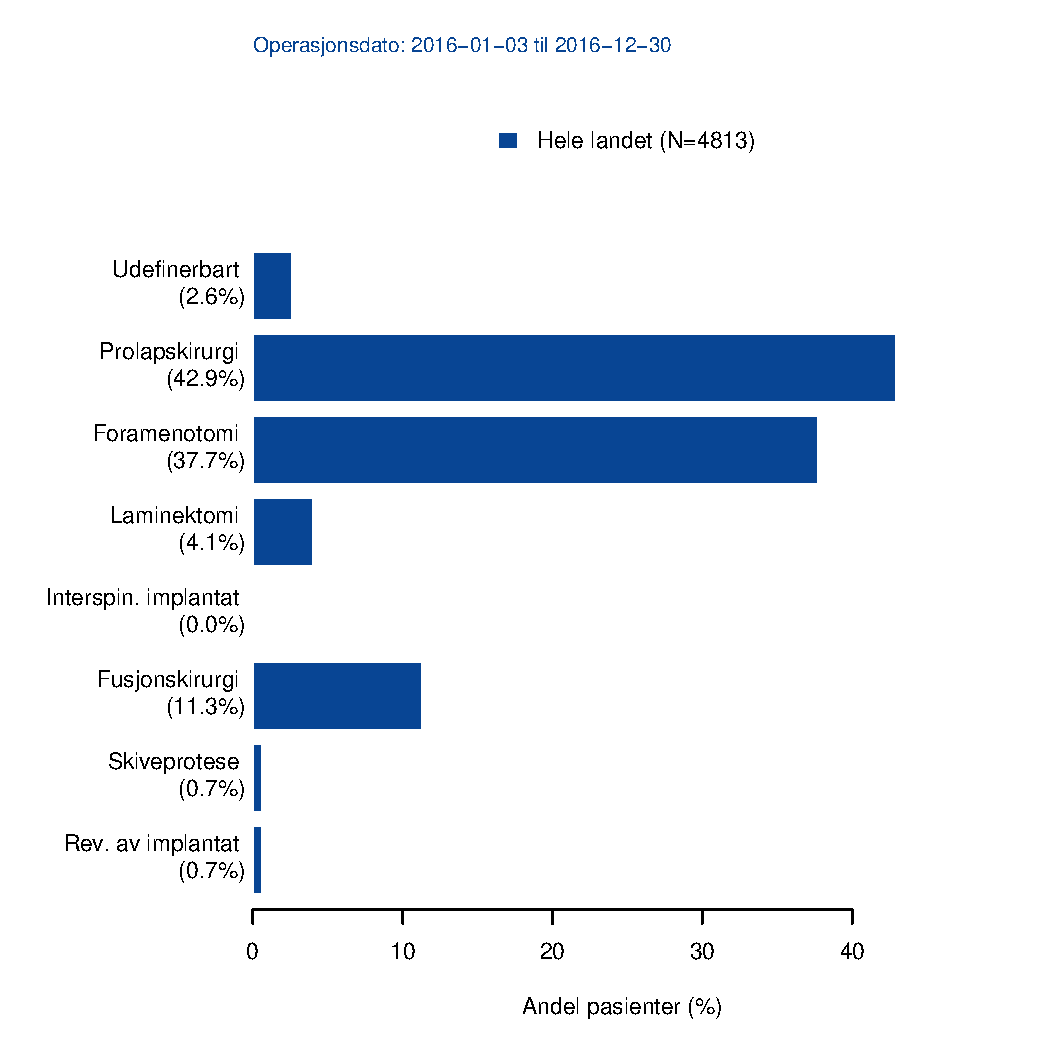
\includegraphics[width= 0.8\textwidth]{HovedInngrep.pdf}
	\caption{\label{fig:HovedInngrep} Hovedinngrep.}
\end{figure}





\subsection{Liggetid}

Informasjonen er hentet fra legeskjema.
Figur \ref{fig:Liggedogn} viser gjennomsnittlig antall liggedøgn per år og fordeling av liggedøgn. 
%for pasienter operert ved shtxt og landet for øvrig.





\begin{figure}[h] 
\centerline{
  \scalebox{0.5}{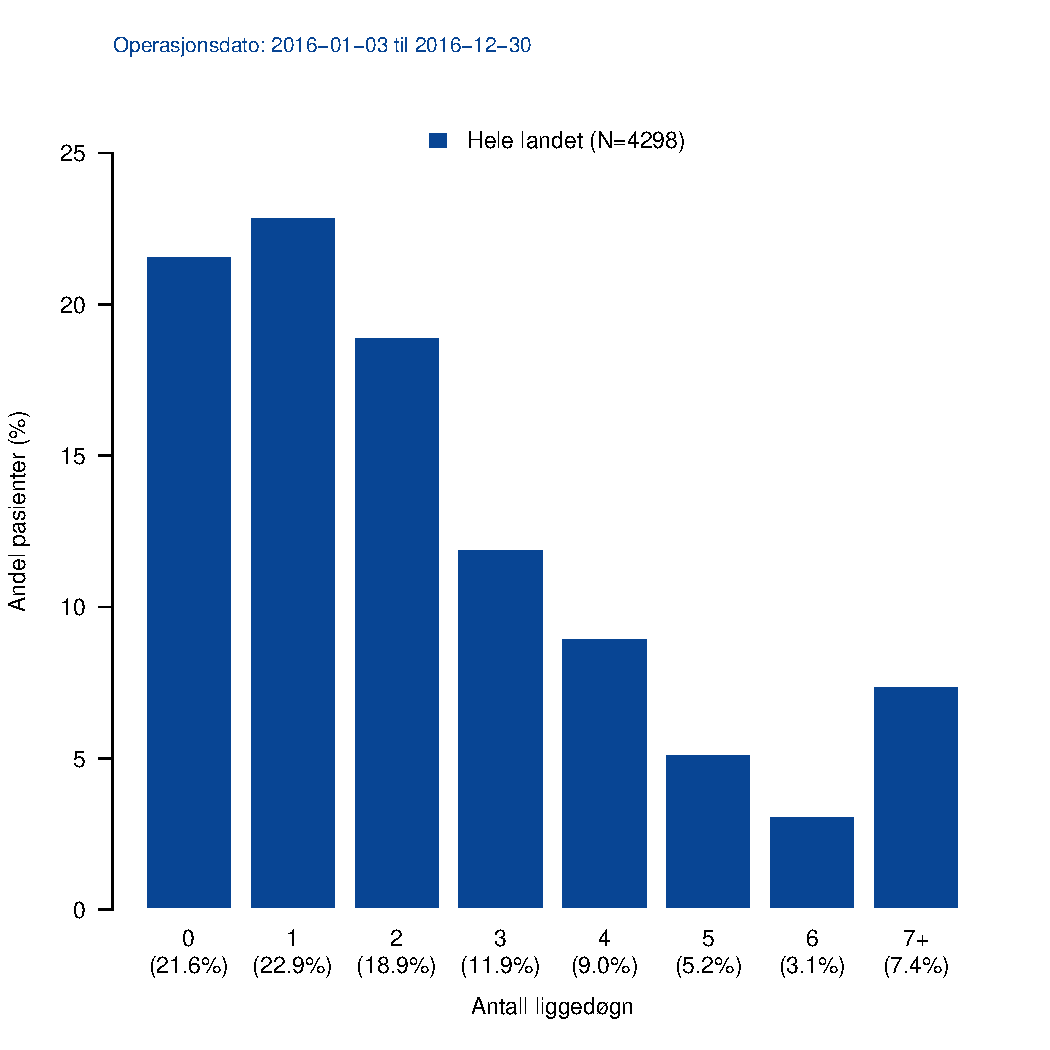
\includegraphics{FigLiggetidFord.pdf}}
  \scalebox{0.5}{\includegraphics{LiggetidBox.pdf}}
  }
  \caption{Liggetid ved operasjon.}
  \label{fig:Liggedogn}
\end{figure}






\subsection{Prescore}

Pasientene som i utgangspunktet har mye plager, vil kunne forvente størst gevinst av en operasjon, 
mens de som har lite plager vil ha mindre potensial for forbedring og større risiko for 
forverring (”tak- og gulveffekter”). Det vil si at en stor del av variasjonen når det gjelder 
utkomme etter kirurgi, henger sammen med hvor streng indikasjonsstillingen har vært.

Figur \ref{fig:Pre} viser score av EQ-5D, Oswestry Disability Index(ODI), 
smerter i bein og rygg før operasjon, dvs. hvor dårlig fysisk funksjon og sykdomsspesifikk 
livskvalitet var.
Prescore gir en pekepinn på hvor streng operasjonsindikasjonen har vært.






\begin{figure}[h] 
\centerline{
  \scalebox{0.5}{\includegraphics{EQ5DPre.pdf}}
  \scalebox{0.5}{\includegraphics{OswPre.pdf}}
	}
  \centerline{
  \scalebox{0.5}{\includegraphics{SmBePre.pdf}}
  \scalebox{0.5}{\includegraphics{SmRyPre.pdf}}
  }
  \caption{Prescore for hhv. EQ-5D, ODI, bein- og ryggsmerter.}
  \label{fig:Pre}
\end{figure}


\clearpage

\section{Resultatmål}
All informasjon i dette kapitlet er hentet fra pasientskjema. Ingen av resultatmålene er justert
for eventuelle ulikheter i pasientpopulasjonene.


\subsection{Effekt av operasjon kontra prescore}
Figur \ref{fig:EndrPre} viser sammenhengen mellom prescore og endring i de ulike effektmålene.





\subsection{Oswestry Disability Index (ODI)}
ODI er en score for fysisk funksjon og et sykdomsspesifikt livskvalitetsmål. Skalaen går fra 0
til 100, hvor 0 angir ingen funksjonshemming og følgelig beste livskvalitet.
Figur \ref{fig:OswEndr} viser fordeling av ODI før og etter operasjon.
Figur \ref{fig:OswEndrSml} viser andel pasienter med klinisk signifikant forbedring av ODI (dvs. minst 30$\%$) 12 mnd. etter operasjon. Høyre del av figuren viser gjennomsnittlig endring hos pasienter operert ved NKR 12 måneder
etter operasjon sammenliknet med landet for øvrig og de tre avdelingene/sykehusene som har 
med størst forbedring i ODI. Merk at resultatene \textit{ikke} justert for forskjeller i pasientpopulasjonene.




 

\begin{figure}[h] 
\centerline{
  \scalebox{0.8}{\includegraphics{OswEndr.pdf}}
  }
  \caption{Figuren viser gjennomsnittlig endring i Oswestry, 12 mnd. etter operasjon, per år.}
  \label{fig:OswEndr}
\end{figure}


\subsection{EQ-5D}
EQ-5D er et generelt livskvalitetsmål, tradisjonelt benyttet av helseøkonomer, men det har også
vist seg å fungere som livskvalitetsmål i ryggkirurgi. Skalaen går fra -0.6 til 1, hvor lav verdi
angir lav livskvalitet.


\begin{figure}[h] 
\centerline{
  \scalebox{0.5}{\includegraphics{EQ5DEndrTid1.pdf}}
  \scalebox{0.5}{\includegraphics{EQ5DEndrTid2.pdf}}
  }
  \caption{Endring i EQ-5D, 12 mnd.etter operasjon}
  \label{fig:EQ5DEndr}
\end{figure}

Figur \ref{fig:EQ5DEndr} viser endring i EQ-5D score 3 og 12 mnd. etter operasjon. 
%hos pasienter operert ved shtxt og i landet for øvrig for hvert år.


\subsection{Rygg- og beinsmerter}
Skala for rygg-/beinsmerter går fra 0 til 10, hvor 0 betegner ingen smerte.



\begin{figure}[h] 
\centerline{
  \scalebox{0.5}{\includegraphics{SmRyggEndrPre.pdf}}
  \scalebox{0.5}{\includegraphics{SmRyggEndrTid.pdf}}
  }
  \caption{Endring i ryggsmerter, 12 mnd.etter operasjon}
  \label{fig:SmRygg}
\end{figure}

Figur \ref{fig:SmRygg} endring av ryggsmerter fra før til etter operasjon, samt endring i ryggsmerter.




\begin{figure}[h] 
\centerline{
  \scalebox{0.5}{\includegraphics{SmBeinEndrPre.pdf}}
  \scalebox{0.5}{\includegraphics{SmBeinEndrTid.pdf}}
  }
  \caption{Endring i beinsmerter, 12 mnd.etter operasjon}
  \label{fig:SmBein}
\end{figure}

Figur \ref{fig:SmBein} viser differansen av ryggsmerter fra før til etter operasjon.


\clearpage


\subsection{Opplevd nytte av operasjon}

Figur \ref{fig:Nytte} viser hvor stor nytte pasientene opplever å ha hatt av behandlingen 12 mnd. etter operasjon ved NKR fordelt på år. Det hvite merket på søylene angir andel pasienter som angir at de har blitt ''Frisk'' eller ''Mye bedre'' i landet for øvrig . Tallet øverst på søyla angir antall pasienter som har svart. 
I figuren er det gjort følgende aggregering av svaralternativene i spørreskjemaet:
\begin{itemize}
	\item ''Frisk mye/bedre'' omfatter ''helt bra'' og ''mye bedre'' 
	\item ''Omtrent uendret'' omfatter ''litt bedre'', ''ingen endring'' og ''litt verre'' 
	\item ''Klart verre'' omfatter ''mye verre'' og ''verre enn noen gang før''
\end{itemize}



\begin{figure}[h] 
	\begin{center}
  \scalebox{0.8}{\includegraphics{FigNytte.pdf}}
	\end{center}
  \caption{Hvilken nytte mener du at du har hatt av operasjonen?, (12 mnd etter operasjon)}
  \label{fig:Nytte}
\end{figure}




\subsection{Pasienttilfredshet}

Figur \ref{fig:Fornoyd} viser hvor fornøyde pasientene er 12 mnd. 
etter operasjon fordelt på år. (\textbf{Her må det være feil i datagrunnlaget...} Det hvite merket på søylene angir andel fornøyde pasienter i landet for øvrig. Tallet øverst på søyla angir antall pasienter som har svart. 


\begin{figure}[h] 
	\begin{center}
\scalebox{0.8}{\includegraphics{FigFornoyd.pdf}}
	\end{center}
  \caption{Hvor fornøyd er du med behandlinga du har fått på sykehuset?, 12 mnd etter operasjon}
  \label{fig:Fornoyd}
\end{figure}


\end{document}
